\chapter{Introduction}

\section{The Rise of Digital Identity Wallets and the Need for Secure, Private, Usable Solutions}
Digital credential wallets, the digital analogue of their physical counterparts, are emerging as essential tools for identity verification in both online and offline contexts. Nations such as India, Singapore, South Korea, Estonia, and Norway have implemented nationwide digital identity systems, while the EU mandates adoption across member states by 2026, and the US advances pilots in 13 states.  These systems aim to streamline identity management, yet their success depends on resolving a fundamental trilemma: ensuring privacy, security, and usability. Consider the following scenarios

\begin{enumerate}
    \item \textbf{KYC/AML Bank Application}: Opening a bank account requires verifying citizenship, age, government issued credentials, and possibly financial standing (bank balances). Traditional KYC processes are slow and complex, with up to 68\% of users abandoning applications, with additional privacy risks of sharing and storing user personal information

    \item \textbf{Social Media Verification:} Accessing social media in Australia will soon require age (over 16) and citizenship verification. A frequent transaction that could leak a childs online movements 

    \item \textbf{Age and Health Status: } Interacting with a medical clinic often requires different criteria to be met, such as a vaccination status, age, insurance status. Current processes require a user to show all information during the process. 
\end{enumerate}

Across these cases, users seek privacy; disclosing only essential information—while verifiers require security, such as authenticity and fraud resistance. Usability demands rapid, cross-device verification of multiple, hetereogenous credentials. Yet, prior systems falter: they expose excessive data, fuel cybercrime, and lack efficiency. The previous generation of anonymous credential frameworks \cite{hutchison_signature_2004, hutchison_constant-size_2006, sako_short_2016}, though innovative, met basic needs—verifying a single credential in 50ms—but fail to address the complex, multi-credential demands of the next generation of identity systems. Verifying multiple credentials is either too slow, lack a theoretical framework and security properties, or lack efficient and private mechanisms for sybil resistance and revocation. These gaps are already driving discussions at the Internet Identity Workshop \cite{internet_identity_workshop_internet_2025} and looking for solutions.

This thesis develops cryptographic primitives to enable digital credential wallets that are fast, private, and resilient to abuse, paving the way for advanced identity solutions that transcend current limitations and unlock new functionality for secure and private digital interactions.


\section{Anonymous Credentials}
Anonymous credential systems enable privacy-preserving authentication and access control, allowing users to prove specific attributes without revealing their full identity. Anonymous Credentials is the base building block of digital credential wallets, where users manage diverse credentials (e.g., passports, bank statements) to verify identity across scenarios like KYC or age verification. They fulfill two primary roles: ensuring holder authenticity like signature verification (e.g., proving knowledge of a secret key) and enforcing access control (e.g., demonstrating eligibility based on attributes like age $ > 21 $).

The Anonymous Credential framework involves three main actors: the \emph{user}, who owns the credential wallet with credentials, their attributes, and their signing/verification keys; the \emph{issuer}, who creates credentials; and the \emph{verifier}, who checks them. Credentials are authenticated data structures that cryptographically bind attributes, ensuring both hiding (privacy) and binding (security). These structures vary by issuance model and underlying cryptographic primitive. Credentials could be issued by a single-issuer as most are issued today, or to protect against malicious issuers, it could be threshold of issuers or even blockchain-based smart contracts. Credentials could be in the form of signatures or even data-structures in a cryptographic accumulator. The choice of cryptographic data structure dictates the proof system, the proof expressiveness, and the verification efficiency.


\begin{figure}
    \centering
        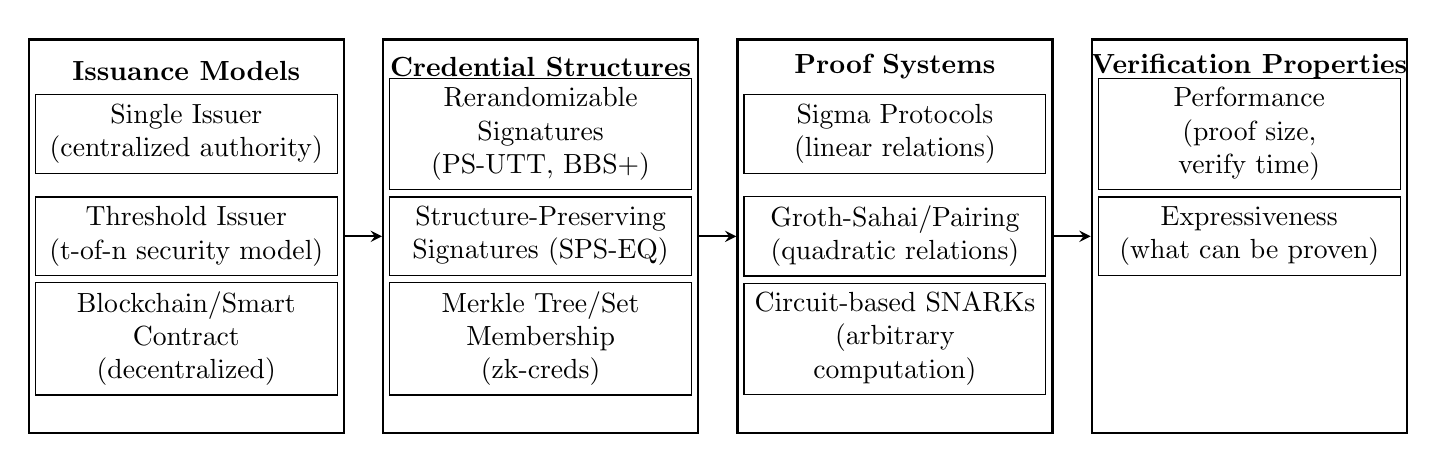
\begin{tikzpicture}[
            box/.style={
                rectangle,
                draw=black,
                thick,
                minimum width=4cm,
                minimum height=5cm,
            },
            title/.style={
                rectangle,
                draw=none,
                thick,
                minimum width=3.8cm,
                minimum height=1cm,
                align=center,
                font=\bfseries
            },
            item/.style={
                rectangle,
                draw=black,
                text width=3.6cm,
                minimum height=1cm,
                align=center
            },
            arrow/.style={->, >=stealth, thick}
        ]
        
        % Outer boxes
        \node[box] (box1) at (0,0) {};
        \node[box] (box2) at (4.5,0) {};
        \node[box] (box3) at (9,0) {};
        \node[box] (box4) at (13.5,0) {};
        
        % Box titles - removed draw=black
        \node[title] (t1) at (0,2.1) {Issuance Models};
        \node[title] (t2) at (4.5,2.15) {Credential Structures};
        \node[title] (t3) at (9,2.15) {Proof Systems};
        \node[title] (t4) at (13.5,2.15) {Verification Properties};
        
        % Connecting arrows
        \draw[arrow] (box1.east) -- (box2.west);
        \draw[arrow] (box2.east) -- (box3.west);
        \draw[arrow] (box3.east) -- (box4.west);
        
        % Items for box 1 - removed bullet points and centered text
        \node[item] (i11) at (0,1.3) {Single Issuer\\(centralized authority)};
        \node[item] (i12) at (0,0) {Threshold Issuer\\(t-of-n security model)};
        \node[item] (i13) at (0,-1.3) {Blockchain/Smart Contract\\(decentralized)};
        
        % Items for box 2 - removed bullet points and centered text
        \node[item] (i21) at (4.5,1.3) {Rerandomizable Signatures\\(PS-UTT, BBS+)};
        \node[item] (i22) at (4.5,0) {Structure-Preserving\\Signatures (SPS-EQ)};
        \node[item] (i23) at (4.5,-1.3) {Merkle Tree/Set Membership\\(zk-creds)};
        
        % Items for box 3 - removed bullet points and centered text
        \node[item] (i31) at (9,1.3) {Sigma Protocols\\(linear relations)};
        \node[item] (i32) at (9,0) {Groth-Sahai/Pairing\\(quadratic relations)};
        \node[item] (i33) at (9,-1.3) {Circuit-based SNARKs\\(arbitrary computation)};
        
        % Items for box 4 - removed bullet points and centered text
        \node[item] (i41) at (13.5,1.3) {Performance\\(proof size, verify time)};
        \node[item] (i42) at (13.5,0) {Expressiveness\\(what can be proven)};
        
        \end{tikzpicture}
        
  
    \caption[Anonymous Credential Framework Diagram]{Anonymous Credential Framework. The Issuance Model determines the Credential Type. The Credential Structure and underlying commitment determines the Proof System and Verification Properties}
    \label{fig:chap1_anon_cred_framework}
\end{figure}



Two core interactive processes govern anonymous credentials. In the \emph{obtain/issue} phase, users commit attributes, and issuers sign them, often blindly to preserve a user's privacy. In the \emph{show/verify} phase, users rerandomize credentials and generate zero-knowledge proofs to meet dynamic verification requirements (e.g., proving $ \text{age} > 16 $ without disclosing birthdate). Verifiers check these proofs for validity. Proof systems, such as Sigma protocols, Groth-Sahai, pairing-based methods or zk-SNARKS, balance expressiveness (e.g., proving complex predicates) with efficiency.

% <<INSERT USER INTERACTING WITH ALL SORTS OF ISSUERS HERE E.g. credential oracles>>
% <<INSERT USER SHOWING + VERIFYING>>

Security hinges on two main properties: \emph{unforgeability}, ensured by the binding nature of commitments and soundness of proofs, and \emph{anonymity}, achieved through hiding commitments, homomorphism of randomizing actions and the zero-knowledge property of zero-knowledge proofs, preventing linkability across verifications. However, designing systems that scale to multi-credential wallets, resist abuse, and perform efficiently involves trade-offs in privacy, efficiency, and expressiveness. These challenges highlight the need for careful selection of combining the fastest cryptographic primitives or optimizing the existing primitives to minimize computational overhead, selecting the most expressive schemes to enable the use-case functionality that is needed for next-generation identity systems.
This Thesis addresses each of these and demonstrates our state-of-the-art primitives via qualitative and quantitiave analysis. 


\section{Gap Analysis}

\subsubsection{Limitation 1: Fast Anonymous Credentials (under 100ms) }

Anonymous credentials fundamentally operate slower than traditional signature schemes like ECDSA which has long limited their adoption. Benchmarks \cite{habib_evaluation_2016} have shown $\mathsf{Show + Verify}$ time for Anonymous Credential systems IBM's Idemix to be $(110ms, 220ms, 450ms)$ for 1,2,3 credentials, Microsoft's U-Prove to be $(180ms, 460ms, 600ms)$ for 1,2,3 credentials respectively, IRMA \cite{fischer-hubner_towards_2013} at $1300ms$ and zk-creds at $465ms$ \cite{rosenberg_zk-creds_2022}. Consider Alice approaching a turnstyle for the train needing to verify her transport ticket and student status. Non-private signatures would sign and verify under $1ms$, whereas current anonymous credentials benchmarks are beyond the $100ms$ rule applied by user experience experts \cite{jakob_nielsen_powers_2009} and threshold for revenue loss due to  at Google and Amazon \cite{linden_geeking_2006}. The consequence is users and system architects prioritizing efficiency over privacy and using non-private methods of authentication. 


\subsubsection{Limitation 2: Security Against Malicious Issuers}
Most Anonymous Credential systems deployed today assume honest-but-curious issuers rather than actively malicious ones; such systems claim strong security and privacy guarantees but fail to recognize the threat from maliciously generated signing and verification keys which could allow a signer to secretly embed tracking or de-anonymising algebraic structure into the credential. This would undermine the systems privacy guarantees and prevent widespread adoption. 


\subsubsection{Limitation 3: Efficient Expressive Proofs}
Definition of Limitation: 
Concrete Example:
Technical Cause
Practical Consequences:


\subsubsection{Limitation 4: Security Verifying Multiple Credentials}
Definition of Limitation: 
Concrete Example:
Technical Cause
Practical Consequences:


\subsubsection{Limitation 5: Efficient Nullifiers}
Definition of Limitation: 
Concrete Example:
Technical Cause
Practical Consequences:




\subsubsection{Limitation 6: Efficient Threshold Signatures}
Definition of Limitation: 
Concrete Example:
Technical Cause
Practical Consequences:


\subsubsection{Limitation 7: Efficient, Secure, Privacy-Preserving Threshold Identity System}
Definition of Limitation: 
Concrete Example:
Technical Cause
Practical Consequences:















Previous deployments like IBM's Idemix \cite{camenisch_design_2002} and IRMA \cite{fischer-hubner_towards_2013} based on CL-Signatures \cite{camenisch_design_2002, cimato_signature_2003}, Hyperledger Fabric \cite{androulaki_hyperledger_2018} based on BBS+ \cite{hutchison_constant-size_2006}, Microsoft's U-Prove \cite{dunkelman_formal_2016} based on Brands' signatures \cite{brands_rethinking_2000}, were deployed in pilot programs \cite{dunkelman_formal_2016}, and proved that these systems were secure, private and feature-rich, but inefficient for widespread adoption. Their implementations were based on early constructions we label as "previous generation" and lacked efficient credential verification procedures required for the expected user experience needed for large-scale uptake, which we illustrate below.

\paragraph{IRMA, Idemix and U-Prove: }

IRMA \cite{fischer-hubner_towards_2013} presents the Show+Verify for credential with 3 attributes costs about 1.3seconds (Intel Core i7-8650U CPU with 16 GB of RAM GNU/Linux) in \cite{zhang_passo_2021}

\cite{habib_evaluation_2016}: presents a more thorough evaluation of the Show+Verify algorithms:
Idemix presents Show + Verify algorithm for 1,2,3 credentials as 110ms, 220ms, 450ms
U-Prove presents Show + Verify algorithm for 1,2,3 credentials as 180ms, 460ms, 600ms
Furthermore, they show functionality use-case like selective disclosure (400ms for 1 attribute selective disclosure and 670ms for 2 attributes selective disclosure) and committed attribute equality (120ms). 

The gap we see here is that 
- doesn't take batch verification into account.
- selective disclosure costs minimal overhead. (under 1ms)
- attribute equality costing minimal overhead (under 1ms)
- Newer schemes \cite{camenisch_anonymous_2016, tomescu_utt_2022} reduce pairing operations in the signature construction itself, coupled with cryptography library improvements reduce all metrics significantly. 
This hasn't been illustrated properly. 

There is a gap in practical evaluation analysis for newer state-of-the-art constructions which we provide benchmarks for.














% \subsection{Chapter \ref{chap2}}
% Improved Constructions of Anonymous Credentials from New Rerandomizable Signatures. This chapter is motivated by the proliferation of credential wallets and needing to (quickly and privately) verify credentials. 
% In this chapter I formalize security for a variant of the PS signature \cite{sako_short_2016}, from the UTT paper \cite{tomescu_utt_2022}, I improve it by making it more efficient and improving security (against malicious issuers) and empirically show it is best in class with concrete benchmarks. 


% \subsection{Chapter \ref{chap3}}
% Identity Binding Multi Issuer Multi Credential Anonymous Credentials. This chapter is motivated by thinking about what's required from credential wallet architecture to verify multiple credentials together. E.g., you have a driver's license, passport, and bank information in your credential wallet, and need to verify it together and prove it's from the same person. I create the security property "Identity Binding" for this situation. I show benchmarks for two different scenarios, 1) the cost of privacy, 2) the improvement from single issuer.
% 1) I compare the two scenarios, verifying credentials without privacy and with privacy and show that privacy preserving credentials doesn't cost much more (in overhead), not what it used to. 2) Our anonymous credential from \ref{chap2} can be aggregated if signed with the same key. I show the efficiency benefit if this is the case. 

% \subsection{Chapter \ref{chap4}}
% New Nullifier Constructions from the $q$-DDHI and Applications to Accountable Privacy Systems. A nullifier is a cryptographic object, similar in thought to a signature. It's created by someone, contains a user's secret key and a specific message, and is given to a verifier to prove that the user made the nullifier with a specific message and they own the key public key that did it. A user who spends their coin would make a nullifier from their secret key and the coin's serial number (like in zcash) and give it the bank to be able to spend it. In Anonymous Credentials, a nullifier ensures a user who requests a credential can't request another one, preventing sybil attacks, which is difficult to do when credentials are private and rerandomizable.
% In accountable privacy, nullifiers should be private, so they shouldn't share the public key. 
% I create New Nullifiers from a series of zero-knowledge proof protocols I made. Starting with a non-private one but a faster version of a VRF \cite{hutchison_verifiable_2005}, and then two nullifier constructions. We will use this for Sybil-resistant anonymous credentials. We show ours are super quick and simple compared to the current.

% \subsection{Chapter \ref{chap5}}
% Sybil Resistant Threshold Issued Identity System from Anonymous Credentials and Anonymous Nullifiers. In this chapter I add threshold-issuance for credentials and build a sybil-resistant private threshold-issued identity system drawing on the work from \ref{chap2, chap3, chap4} and show it's way more efficient than the other state of the art.

% \subsection{Chapter \ref{chap6}}
% Anonymous Credentials Open Source Library - the literature and industry has a gap in implementations for gathering evaluation data for many of these schemes and thus it's hard to determine whether a new scheme has made an improvement or is just using a different technique. I built a few schemes and found many small tricks in the cryptography library make a big difference in concrete implementation efficiency, probably more difference than many "new" papers make theoretically. I wanted to represent this in the Thesis and open-source that for people to use and see.


















What are the theme's we're seeing? 

Firstly, SSI is becoming mainstream. There are implementations from Microsoft, Amazon, 
There are mature standards, the EU is moving ahead to mandate this. they've been doing pilots, building infrastructure, they have over 20 usecases for this
Argentina or someone is using credential wallets on-chain. India has been using a credential wallet for some time. 
This is magnificent. We have the technology primitives and standards.
But what's next? What happens when we move to this? 
Is the cryptography ready? 
Will users experience a feature gap? Is there any effieincy concerns? 
What are the upsides? - the upsides for users is having credentials in one place, potentially connected. Verifying identity will be fast, and private. Reduced data breaches as you will hold your data rather than your data being held on any number of external services. The upsides for businesses is that for e.g. identity verification is fast, they don't hold user information. 

We focus our research on preparing the industry for the next step.
1. efficient credential use. Just building the most efficient credential for the Show+Verify. Using the most efficient and expressive proofs so users can privately prove their attributes. and keeping their things secure.
2. next we focus on a use-case, identity verification for complex verification scenarios where a multitude of credentials might be needed where a user has heaps of credentials in their wallets. How we can think about security in this model, we thought about it and came up with identity binding security property. Then we demonstrated how fast it is to verify many credentials together, both publicly, and privately showing the cost of adding privacy really isn't much. 
3. We built the fastest nullifiers which enable these private systems to be sybil resistant, meaning a user can't get more than 1 credential for a given context. This is surprising hard when the credential is anonymous, so we created novel protocols to hide the inputs and optionally hide the outputs but still enable provable uniqueness with hidden values.
4. We strengthen the security of our credential with threshold issuance, then built a threshold issued identity system with our previous enhancements and show it's really best in class for security, privacy, and efficiency. 
5. all work was open sourced as an open source library, primarily to show these primitives and etc. 


\section{The Privacy-Security-Usability Challenge}
Digital identity systems today face a fundamental trilemma: balancing privacy protection, security guarantees, and practical usability. Consider the everyday scenario of proving you're over 21 at a venue:

Privacy: You shouldn't need to reveal your exact birthdate, name, or address
Security: The venue must be certain the credential is authentic and belongs to you
Usability: Verification should be quick, work across devices, and require minimal technical knowledge

Anonymous credentials resolve this trilemma by allowing users to prove specific attributes without revealing others or enabling tracking. However, their design requires navigating complex trade-offs across four critical components:

\section{The Anonymous Credential Framework}
% What is the role of an Anonymous Credential
Anonymous Credentials have two main roles: first, to verify the authenticity of the holder. Second is access control, what rights does this user or service or bot have. Authenticity is generally determined by a successful authentication, for example, a user with a credential proves they know the secret key by giving their public key. Or the user can prove they know the Merkle proof and the root of their membership in a merkle tree. 

% Who are the main actors?
There are three main actors in an Anonymous Credential System, a User, an Issuer, and a Verifier. 
The user has attributes wanting to be put in a credential, (or the issuer has them), the issuer issues the credential, and the verifier verifies it. 

% What are the main components?
The Anonymous Credential itself has four main components, which we illustrate here for clarity and to put our contributions into perspective. 

A credential proves authentication and access control to a verifier. 
There are usually two processes when verifying attribute-based credentials. 

The Credential itself is an authenticated data structure that cryptographically binds a user's attributes and hides them from the world. The data structure can be authenticated in different ways. For example, it can be in the format of a signature from an authority which can be "blind"-issued, meaning the issuer doesn't see the attributes but can sign without seeing and optionally be proven certain relations exist in the hidden attributes. Additionally, in a decentralized setting where a system wants protection against a set of malicious nodes, signatures can be threshold issued to avoid such fate.
Credentials may be in the form of an accumulator, a different authenticated data structure. The accumulator may be hosted by a blockchain, users proving set membership in the accumulator (or non-membership) may deduce their authentication and their access rights may be proven from the committed data within the authenticated data structure

Anonymous Credentials come in different flavours, each with a different tradeoff. If signatures, signatures can be issued by a single issuer, or a threshold of issuers, or a blockchain. 



% The main Protocol Algorithms / Interactions
Anonymous Credentials have two main algorithm processes.

Obtain, Issue
Obtain is run by a user, the user may prepare the messages for their credential. They may "commit" to their attributes, which in our Thesis means they run a commitment algorithm and output a hiding and binding cryptographic commitment. 

Issue is run by an issuer, a threshold of them, or even in the case of zk-creds, it's blockchain/smart contract operating a merkel tree.


The magnificent thing about anonymous credentials and zero-knowledge proofs is the fact that verification can be somewhat dynamic. The verifier creates a verification statement requirement, such as "the user has a valid credential, their age is over 21, their expiry is bigger than today, etc". The user can generate their proofs in accordance to the criteria while also hiding their credentials. 

Show is an algorithm run by a user to prepare their credential/s for verification. For a signature-based credential, this involves rerandomizing, which generates an indistinguishable version of their original signature, which, by some cryptographic miracle (mainly homomorphism of the underlying credential structure as is the case in BBS+, PS, SPS-EQ), the user generates their proof containing whatever is needed to verify the statement. They may also need to prove membership or non-membership of an accumulator in which they will generate the accumulator membership proof and prove, generally in the same computation, that their credential satisfies all relations within the same computation. 

Verify
The verifier receives 



There are many anonymous credential constructions from the literature, each with their own tradeoffs. Most importantly, the choice of anonymous credential determines the authenticated data structure (e.g. the commitment it uses) which determines the proof system compatibility, which determines the expressiveness and efficiency of using the anonymous credential. Which we call the Show+Verify algorithm. 

% How it's secure
The two main security properties in ABCs is that the credential itself must be unforgeable, and the user must be anonymous. 
Unforgeability reduces to the underlying cryptographic primitives, if it's a signature, is the signature unforgeable? But perhaps that's not enough, if it's a multi-attribute, the the authenticated data structure must have its own unforgeable properties. For example, if it's a commitment, then a malicious user changing messages in the commitment could have catastrophic consequences, e.g. a user changing a birthdate with an expiry. So the underlying cryptographic message holder must also have it's own security properties, e.g. in commitments it is binding. Unforgeability also reduces to the soundness of the proof system. We use sigma protocols and the soundness extractor to reduce unforgeability of the anonymous credential. . Or different structures like Anonymous Counting Tokens, or Verifiable Random Functions that meet the same anonymous credential security properties.

Now for Anonymity, a system is defined as Anonymous if an adversary is given one credential and two verification proofs (which both verify successfully) and cannot tell which proof is geninune and which proof is made up. That formally suggests that the proof, when used for a genuine authentication cannot leak information about the user. Anonymity in an attribute based credential generally reduces to the hiding property of a commitment scheme and the zero knowledge 



Issuers
issuers may be single issuers, threshold issuers, or, in the case of the accumulator, even a blockchain/smart contract.
Issuers historically are organisations like the government issuing a passport, the DMV issuing a drivers license. Infact, these are all issuers with cryptographic keys and nowadays all have chips that can be read and verified with public keys. 
Issuers nowadays also include Credential Oracles which are expanding in popularity, modern anonymous credential systems and credential wallets will need to support credential oracles and there are now unique and interesting problems. How to manage a credential wallet with a multitude of heterogenous credentials, some issued by credential oracles, some issued by governments, etc. How to retain accountability of these systems. We look at ways of solving this problem with Identity Binding. 


The credential choice filters down through the commitment choice, the proof system that the commitment can be used with, and thus the expressiveness and efficiency of the proofs themselves. 
Sigma protocols are proofs of the relations of exponents and are extremely efficient and can be used for many credential requirements like . The proof system limits the computation that can be achieved, with sigma protocols, the exponent must be used, and the exponent must be extractable for reducing the scheme securely. Therefore, algebraic-free computation like a hash function, or anything using a hash primitive for messages generally can't be used. For such extensions, zk-SNARKS trade efficiency with general computation compatibility. However, we focus on the efficient requirements of operating a credential wallet with the efficiency, usability. 
Groth Sahai or pairing based proofs are generally optimised for set membership because of the pairing-based nature of accumultaors but can also be incorporated with sigma protocols with some overhead. SPS-EQ and those type of credentials use set commitments and pairing-based proofs 

zk-SNARKS 




\subsection{Credential Issuance}
\begin{itemize}
    \item 
    \item Single Issuer, Threshold Issuers, Blockchain/Smart Contract
    \item Anonymity against malicious issuers
    \item 
\end{itemize}


\subsection{The Credential Structure}
How attributes are cryptographically bound to an Authenticated Data Structure.
How this impacts the choice of Proof System, which impacts the expressiveness and efficiency
\begin{itemize}
    \item Pedersen Commitments
    \item Polynomial/Set Commitments
    \item Hashed Commitments 
\end{itemize}


\subsection{The Proof System}
\begin{itemize}
    \item Proving Validity of the Authenticated Data Structure
    \item Sigma, Pairing-based, 
\end{itemize}

: The privacy-efficiency-expressiveness triangle


\subsection{Use Cases}

Credential Wallet
Using multiple heterogenous credentials together
Generating nullifiers from anonymous credentials for sybil resistance
Threshold Issuance

Gap Identification

- Cross-credential proofs with efficiency
- Efficiency challenges of previous anonymous credential constructions (especially when considering in the new world we might be verifying multiple credentials together)
- Heterogeneous issuer trust models: Managing credentials from different trust frameworks
- 


My Contributions

\begin{figure}
    \centering
        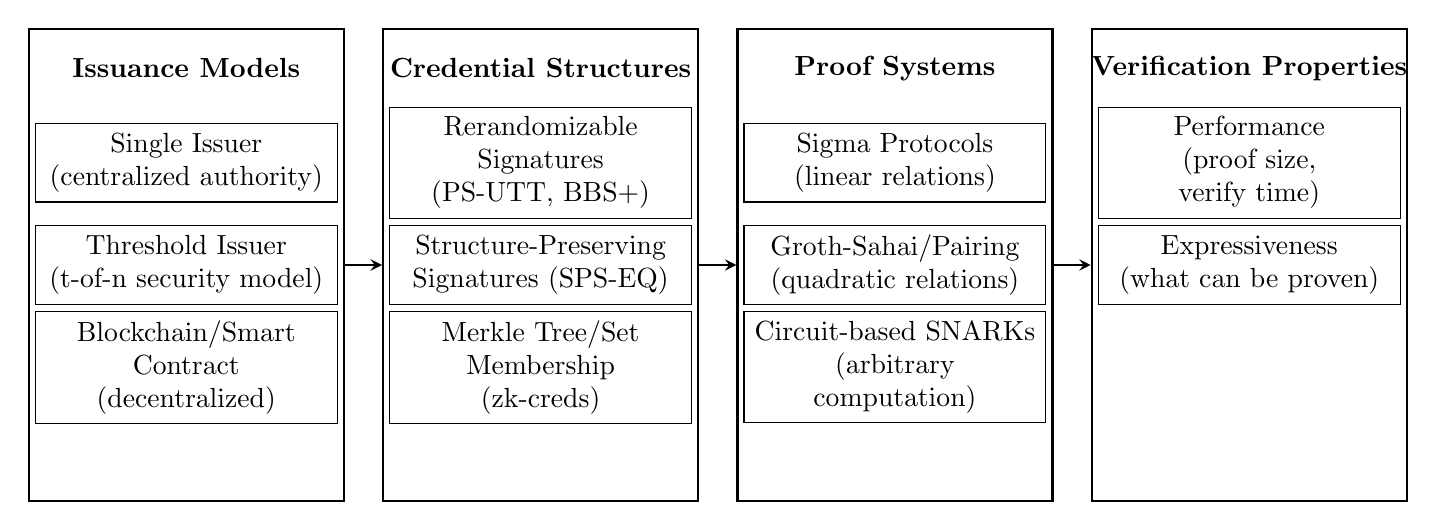
\begin{tikzpicture}[
            box/.style={
                rectangle,
                draw=black,
                thick,
                minimum width=4cm,
                minimum height=6cm,
            },
            title/.style={
                rectangle,
                draw=none,
                thick,
                minimum width=3.8cm,
                minimum height=0.7cm,
                align=center,
                font=\bfseries
            },
            item/.style={
                rectangle,
                draw=black,
                text width=3.6cm,
                minimum height=1cm,
                align=center
            },
            arrow/.style={->, >=stealth, thick}
        ]
        
        % Outer boxes
        \node[box] (box1) at (0,0) {};
        \node[box] (box2) at (4.5,0) {};
        \node[box] (box3) at (9,0) {};
        \node[box] (box4) at (13.5,0) {};
        
        % Box titles - removed draw=black
        \node[title] (t1) at (0,2.5) {Issuance Models};
        \node[title] (t2) at (4.5,2.5) {Credential Structures};
        \node[title] (t3) at (9,2.5) {Proof Systems};
        \node[title] (t4) at (13.5,2.5) {Verification Properties};
        
        % Connecting arrows
        \draw[arrow] (box1.east) -- (box2.west);
        \draw[arrow] (box2.east) -- (box3.west);
        \draw[arrow] (box3.east) -- (box4.west);
        
        % Items for box 1 - removed bullet points and centered text
        \node[item] (i11) at (0,1.3) {Single Issuer\\(centralized authority)};
        \node[item] (i12) at (0,0) {Threshold Issuer\\(t-of-n security model)};
        \node[item] (i13) at (0,-1.3) {Blockchain/Smart Contract\\(decentralized)};
        
        % Items for box 2 - removed bullet points and centered text
        \node[item] (i21) at (4.5,1.3) {Rerandomizable Signatures\\(PS-UTT, BBS+)};
        \node[item] (i22) at (4.5,0) {Structure-Preserving\\Signatures (SPS-EQ)};
        \node[item] (i23) at (4.5,-1.3) {Merkle Tree/Set Membership\\(zk-creds)};
        
        % Items for box 3 - removed bullet points and centered text
        \node[item] (i31) at (9,1.3) {Sigma Protocols\\(linear relations)};
        \node[item] (i32) at (9,0) {Groth-Sahai/Pairing\\(quadratic relations)};
        \node[item] (i33) at (9,-1.3) {Circuit-based SNARKs\\(arbitrary computation)};
        
        % Items for box 4 - removed bullet points and centered text
        \node[item] (i41) at (13.5,1.3) {Performance\\(proof size, verify time)};
        \node[item] (i42) at (13.5,0) {Expressiveness\\(what can be proven)};
        
        \end{tikzpicture}
        
  
    \caption{Caption}
    \label{fig:enter-label}
\end{figure}







\section{Use Case}
One overarching use case is a user and their credential wallet.
Component specific examples

Issuance Models: Show how the wallet must handle credentials from centralized authorities (government), threshold systems (university consortium), and blockchain (professional certification) - highlighting compatibility challenges
Credential Structures: Demonstrate how different credential formats create storage and management challenges when a user needs to prove "identity + qualification + certification" in a single transaction
Proof Systems: Illustrate the complexity when a user needs to prove "I'm over 21, qualified in field X, and certified by organization Y" across heterogeneous credentials
Verification Properties: Show performance bottlenecks when verifying multiple credentials on mobile devices with battery/processing constraints

Gap Identification - where my chapters fit into the 4 blocks

Scale challenges: Traditional systems weren't designed for wallets managing dozens or hundreds of credentials
Cross-credential proofs: The need to prove statements across different credential types
Efficiency on constrained devices: Mobile-first verification requirements
Heterogeneous issuer trust models: Managing credentials from different trust frameworks
















% # High-Level Feedback on Component-Based Introduction Structure

% Your approach using component-based introduction with use cases is excellent - it makes abstract cryptographic concepts accessible while establishing a clear taxonomy. Here's my feedback:

% ## Strengths of Your Approach
% - Using framework components as subheadings creates perfect alignment with your diagram
% - Concrete use cases will help ground theoretical concepts
% - The 4-part structure creates a natural progression from issuance to verification

% ## Suggested Enhancements

% 1. **Start with a practical motivating scenario** before introducing the framework - perhaps a brief vignette showing the privacy challenges in digital identity that anonymous credentials solve

% 2. **Add interconnection emphasis** - explicitly show how choices in one component constrain or enable options in subsequent components (e.g., how blockchain issuance naturally leads to certain credential structures)

% 3. **Include tension points** - highlight the fundamental trade-offs between privacy, efficiency, and expressiveness that drive design choices across components

% 4. **Create a clear transition bridge** between your framework introduction and your contributions - identify specific gaps in existing approaches that your work addresses

% ## Structure Recommendation

% 1. **Opening Problem Statement**: Digital identity privacy challenges
% 2. **Framework Introduction**: Brief overview of the four components
% 3. **Component Deep Dives**: (Your subheadings)
%    - **Issuance Models**: From centralized to decentralized trust
%    - **Credential Structures**: How attributes are cryptographically bound
%    - **Proof Systems**: The privacy-efficiency-expressiveness triangle
%    - **Verification Properties**: What guarantees can be achieved
% 4. **System Taxonomy**: Show how existing systems map to your framework
% 5. **Gap Identification**: What combinations remain underexplored?
% 6. **Your Contributions**: How your work addresses these gaps

% This structure not only introduces anonymous credentials but positions your framework itself as a contribution - a novel way to categorize and understand the design space.







% Gaps Your Thesis Addresses

% Wallet-Centric Architecture Scalability (Ch. 2)

% Traditional schemes weren't designed for managing potentially thousands of heterogeneous credentials
% Your PS-UTT G2 variant achieves 10-16\% faster verification than previous approaches


% Security Against Malicious Issuers (Ch. 2)

% Your key verification protocol prevents deanonymization attacks through maliciously generated keys


% Multi-Issuer Identity Binding (Ch. 3)

% Your MIMC-ABC system enables users to privately combine credentials from multiple issuers while proving they belong to the same identity
% Performance evaluations show multi-issuer verification remains efficient (18.67ms vs. 6.77ms baseline)


% Efficient Privacy-Preserving Sybil Resistance (Ch. 4)

% Your pairing-free Nullifier construction provides 3-6x more efficient nullifiers than existing approaches


% Threshold Sybil-Resistant Identity System (Ch. 5)

% T-SIRIS combines MIMC-ABC and CRBN for threshold issuance with Sybil resistance
% Outperforms S3ID with 44.1× faster verification for large attribute sets


% Proof System Efficiency Beyond Theory (Ch. 6)

% Your benchmark library demonstrates Schnorr protocols achieve sublinear scaling through MSM optimizations











































(To be written properly)
The thesis focuses on improving Anonymous Credentials and specifically for a few use-cases. We will soon be using digital credential wallets (mandated by the EU) \cite{european_parliament_meps_2024} and similar initiatives globally. 


\subsection{Chapter \ref{chap2}}
Improved Constructions of Anonymous Credentials from New Rerandomizable Signatures. This chapter is motivated by the proliferation of credential wallets and needing to (quickly and privately) verify credentials. 
In this chapter I formalize security for a variant of the PS signature \cite{sako_short_2016}, from the UTT paper \cite{tomescu_utt_2022}, I improve it by making it more efficient and improving security (against malicious issuers) and empirically show it is best in class with concrete benchmarks. 


\subsection{Chapter \ref{chap3}}
Identity Binding Multi Issuer Multi Credential Anonymous Credentials. This chapter is motivated by thinking about what's required from credential wallet architecture to verify multiple credentials together. E.g., you have a driver's license, passport, and bank information in your credential wallet, and need to verify it together and prove it's from the same person. I create the security property "Identity Binding" for this situation. I show benchmarks for two different scenarios, 1) the cost of privacy, 2) the improvement from single issuer.
1) I compare the two scenarios, verifying credentials without privacy and with privacy and show that privacy preserving credentials doesn't cost much more (in overhead), not what it used to. 2) Our anonymous credential from \ref{chap2} can be aggregated if signed with the same key. I show the efficiency benefit if this is the case. 

\subsection{Chapter \ref{chap4}}
New Nullifier Constructions from the $q$-DDHI and Applications to Accountable Privacy Systems. A nullifier is a cryptographic object, similar in thought to a signature. It's created by someone, contains a user's secret key and a specific message, and is given to a verifier to prove that the user made the nullifier with a specific message and they own the key public key that did it. A user who spends their coin would make a nullifier from their secret key and the coin's serial number (like in zcash) and give it the bank to be able to spend it. In Anonymous Credentials, a nullifier ensures a user who requests a credential can't request another one, preventing sybil attacks, which is difficult to do when credentials are private and rerandomizable.
In accountable privacy, nullifiers should be private, so they shouldn't share the public key. 
I create New Nullifiers from a series of zero-knowledge proof protocols I made. Starting with a non-private one but a faster version of a VRF \cite{hutchison_verifiable_2005}, and then two nullifier constructions. We will use this for Sybil-resistant anonymous credentials. We show ours are super quick and simple compared to the current.

\subsection{Chapter \ref{chap5}}
Sybil Resistant Threshold Issued Identity System from Anonymous Credentials and Anonymous Nullifiers. In this chapter I add threshold-issuance for credentials and build a sybil-resistant private threshold-issued identity system drawing on the work from \ref{chap2, chap3, chap4} and show it's way more efficient than the other state of the art.

\subsection{Chapter \ref{chap6}}
Anonymous Credentials Open Source Library - the literature and industry has a gap in implementations for gathering evaluation data for many of these schemes and thus it's hard to determine whether a new scheme has made an improvement or is just using a different technique. I built a few schemes and found many small tricks in the cryptography library make a big difference in concrete implementation efficiency, probably more difference than many "new" papers make theoretically. I wanted to represent this in the Thesis and open-source that for people to use and see.

% \subsubsection{Motivation}
% Construct the most efficient and expressive Multi-Show ABC
% SPS-EQ is efficient (don't have concrete benchmarks) but proofs are not as expressive
% ACT is efficient, proofs are expressive but slower, but not malicious issuer secure
% zk-creds is expressive but not as efficient


% \subsubsection{Results/Contributions}
% \begin{enumerate}
%     \item Prove the PSUTT sig excels in the ABC model
%     \item Show it has more functionality than SPS-EQ and TACT and is more efficient than zkSNARK
%     \item Extended the signature with security (anonymity) against malicious issuers
%     \item Our results show we are the most efficient construction.
% \end{enumerate}




% \subsection{Chapter 3}
% \subsubsection{Motivation}
% We can motivate this by the dropout data from online financial applications needing to verify multiple credentials and KYC/AML simultaneously. 
% We show a secure construction to issue and verify credentials together to solve this problem and give benchmarks for different scenarios.
% Introduce Identity Binding security property.

% Construct the most efficient and expressive Multi-Show ABC
% SPS-EQ is efficient (don't have concrete benchmarks) but proofs are not as expressive
% ACT is efficient, proofs are expressive but slower, but not malicious issuer secure
% zk-creds is expressive but not as efficient


% \subsubsection{Contributions}
% \begin{enumerate}
%     \item 
% \end{enumerate}




% % -68\% of consumers abandoned an application – up from 63\% in 2020, 38\% in 2019. Abandonment rate close to 80\% for 25-34 year olds.
% % - 92\% of consumers are concerned about data privacy.





% \subsection{Chapter 2}












% The Internet Identity Workshop discussed a problem space summarised by the following problems:
% \begin{enumerate}
%     \item issuing credentials that are both government and privately issued
%     \item retaining accountability in derived credentials, ensuring derived credentials are fit for purpose and have revocation (Proveable Provenance, Linked Data)
%     \item combining traditional digital identity with decentralized identity
% \end{enumerate}

% A user has an Identity linked to multiple credentials, such as a driver's license and university card. Users want to authenticate with various Relying Parties (Verifiers) without being linked between multiple uses of the same service (e.g. a user verifying multiple credentials with 1 service such as a bank requiring proof of multiple credentials linked to an identity), and between uses of different services (e.g. a user presenting their drivers license for age verification on multiple services).

% Current decentralized identity systems either don't provide this functionality or provide it at the expense of either accountability or privacy. CanDID stores a map between users multi-layered credentials providing a solution to the problem at the expense of the user's privacy. Other credential systems and pseudonym systems prove equality of hidden attributes in a credential such as name or id, which can more-easily be forged and does not support the hierarchical structure leveraging a highly secure and accountable government identity with not-so secure private credentials.









% (sam - speak about the business impact of verifying identity, KYC/AML simultaneously which is what my Thesis is about, e.g. response times / limits https://www.nngroup.com/articles/response-times-3-important-limits/ 



% The rapid digitization of society has elevated digital identity systems to a cornerstone of online trust, processing billions of verifications daily~\cite{noauthor_happy_2021, pang_zanzibar_2019}. Yet, traditional centralized systems, while meeting regulatory needs~\cite{eltayeb_crucial_2024}, are plagued by privacy and security vulnerabilities, with data breaches compromising billions of users~\cite{zhang_data_2022}. The European Union’s eIDAS framework, mandating a digital identity wallet for every citizen by 2026~\cite{noauthor_regulation_2024}, underscores the urgent need for secure, privacy-preserving alternatives. Moving to privacy-preserving digital identities reveals several functionality gaps; tensions between privacy and accountability in identity systems will hinder the functionality expectations of the new digital identity architecture. 

% Decentralized Identity (DID) systems, as outlined by W3C standards, empower users to control their credentials~\cite{soltani_survey_2021}, yet many implementations falter in balancing privacy with accountability~\cite{maram_candid_2020}. Anonymous Credential Systems (ACS) offer a cryptographic solution, enabling privacy-preserving authentication~\cite{chaum_untraceable_1981, hutchison_signature_2004, dunkelman_formal_2016, security_team_computer_science_dept_ibm_zurich_cryptographic_2010}. However, challenges persist in achieving sybil resistance, revocation, and expressive authentication while integrating real-world identity data~\cite{crites_syra_2024, rosenberg_zk-creds_2022}. Current systems either fall short or are inefficient for real-world deployment. 

% This thesis delivers a framework for efficient, secure, and decentralized anonymous credential systems, directly addressing these gaps. We focus on decentralized identity as the primary use case, enabling users to prove attributes across multiple issuers (e.g., combining passports and bank statements) without sacrificing privacy or enabling abuse. Our work builds on prior innovations in credential oracles~\cite{zhang_deco_2020}, which allow individuals to create digital identities from existing real-world credentials—such as passports~\cite{rosenberg_zk-creds_2022} or Web2 logins~\cite{baldimtsi_zklogin_2024}—seamlessly integrating them into privacy-preserving architectures. These advancements are not just timely but essential: without them, emerging frameworks like eIDAS risk deploying vulnerable systems, undermining global digital security.

% Our contributions are five-fold:
% \begin{enumerate}
%     \item \textbf{Optimized Expressive Proofs}: We enhance the PS signature to support efficient zero-knowledge proofs of complex predicates (e.g., AND/OR/Equality, etc), achieving a $5$-$10\%$ speedup over prior constructions while ensuring anonymity against malicious issuers, proven secure in the Algebraic Group Model (Chapter $2$).
    
%     \item \textbf{Multi-Issuer Multi-Credential System (MIMC-ABC)}: We formalize security properties for binding credentials across multiple issuers, constructing a secure system with anonymity guarantees and show illustrate the computational cost of privacy, single issuer, and multi-issuer for a credential system
%     (Chapter $3$).
    
%     \item \textbf{Sybil Resistance}: We introduce multiple novel, pairing-free nullifier schemes that demonstrate speedup ($1.9\times$) and private functionality over existing methods, enabling privacy-preserving accountability (Chapter $4$).
    
%     \item \textbf{Threshold Decentralized Identity}: We design a threshold issuance protocol integrating MIMC-ABC and Sybil Resistance, outperforming comparable systems by xxxx across benchmarks (Chapter $5$).
    
%     \item \textbf{Open-Source Benchmark Framework}: We provide the first standardized toolkit for fair evaluation of ABC schemes, enhancing reproducibility and practical insight (Chapter $6$).
% \end{enumerate}

% % These advancements collectively resolve key tensions between privacy, accountability, and efficiency.  Beyond identity, our framework extends to anonymous credential applications like e-cash and anonymous voting, highlighting its versatility. The thesis is organized as follows: Sections~\ref{sec:commitment} and~\ref{sec:pssignature} detail our cryptographic primitives, Section~\ref{sec:sigmaproofs} presents the sigma protocols, Section~\ref{sec:mimc} describes the MIMC system, Section~\ref{sec:idsys} builds the identity system, and Section~\ref{sec:evaluation} provides our evaluation.




















% \newpage
% \section{Motivation}
% \subsubsection*{Overarching Research Problem: }
% How can we build privacy-preserving credential systems that are simultaneously expressive, efficient, secure against malicious actors, resistant to abuse, and free from centralized trust?


% \subsubsection*{Chapter 2: Foundations: } 
% How can we construct anonymous credential systems that efficiently support expressive proofs—like range proofs, attribute equality, or set membership—while remaining secure against malicious issuers? Existing schemes either verify simple proofs (e.g., possession) efficiently (sps-eq, ACT) or handle complex predicates at high computational cost (zk-creds), often assuming honest issuers (ACT, Coconut). This chapter lays the foundation for a system that overcomes these limitations.

% \noindent \textbf{Technical Challenges}
% \begin{enumerate}
%     \item Designing an Anonymous Credential scheme for efficient zero-knowledge proof of complex predicates without using zkSNARK
%     \item Ensuring security for malicious issuers without affecting performance
%     \item Balancing computational overhead with practical usability
% \end{enumerate}

% \subsubsection*{Chapter 3: Multi-Issuer Multi-Credential System: } 
% How can users privately combine credentials from multiple, mutually distrusting issuers (e.g., government IDs and bank statements) to prove they belong to the same identity, especially in decentralized settings? Non-private systems easily verify credential consistency, but privacy-preserving approaches struggle to bind credentials securely without a trusted party, aggregate signatures \cite{mir_aggregate_2023} have trouble with revoking individual credentials from an aggregate.

% \noindent \textbf{Technical Challenges}
% \begin{enumerate}
%     \item Defining and achieving identity binding across credentials without revealing the user’s identity.
%     \item Preventing attacks where users mix credentials from different identities (e.g., credential swapping).
%     \item Maintaining efficiency as the number of issuers and credentials scales.
% \end{enumerate}



% \subsubsection*{Chapter 4: Sybil Resistance: } 
% How can we prevent Sybil attacks—where users create multiple identities to abuse services like voting or payments—in anonymous credential systems without compromising privacy? Traditional nullifier schemes either leak information or are too costly for multi-issuer scenarios.

% \noindent \textbf{Technical Challenges}
% \begin{enumerate}
%     \item Creating unique, privacy-preserving bindings (e.g., nullifiers) for credentials without a central authority.
%     \item Designing efficient nullifiers that scale to multi-issuer, multi-credential settings.
%     \item Integrating these with zero-knowledge proofs to ensure verification doesn’t reveal identities.
% \end{enumerate}



% \subsubsection*{Chapter 5: Threshold Issuance: } 
% How can we distribute trust in credential issuance to eliminate central points of failure, while preserving the efficiency and security of our anonymous credential system? Centralized issuers risk catastrophic breaches—malicious actors could issue unlimited credentials—yet adapting efficient schemes to a threshold model is complex, especially for multi-credential verification.

% \noindent \textbf{Technical Challenges}
% \begin{enumerate}
%     \item Adapting our efficient signature scheme for threshold key generation and signing.
%     \item Ensuring private, distributed issuance.
%     \item Security against colluding or malicious threshold issuers
% \end{enumerate}

% \section{Contributions and Thesis Organization}

% This thesis develops a comprehensive privacy-preserving digital identity framework that enables expressive credential verification, multi-issuer identity binding, and sybil resistance without compromising efficiency or security. My contributions span four interconnected areas:

% \begin{enumerate}
%     \item \textbf{Foundations: Expressive Predicates for Attribute-Based (Anonymous) Credentials (ABC's)} (Chapter 2)
%     \begin{itemize}
%         \item Extended rerandomizable signature scheme with formal position-binding security in the Algebraic Group Model
%         \item Formalized security model for anonymity against colluding credential issuers
%         \item Developed a G2-variant optimization reducing verification costs by [X\%]
%         \item Demonstrated sub-linear practical performance using multi-scalar multiplication techniques
%         \item Benchmarked predicate proofs against SOTA showing on average [X\%] improvement
%         \item Provided the first comprehensive benchmarks across BBS+ and PS signature variants
%     \end{itemize}

%     \item \textbf{Multi-Issuer Multi-Credential System (MIMC-ABC)} (Chapter 3)
%     \begin{itemize}
%         \item Formalized security model for multi-issuer identity binding with position-binding commitments
%         \item Proved unforgeability and anonymity even against colluding credential issuers
%         \item Demonstrated 30\% performance improvement over comparable schemes for multi-credential verification
%     \end{itemize}
    
%     \item \textbf{Private Accountability: Sybil Resistance} (Chapter 4)
%         \begin{itemize}
%             \item Introduced the Credential Relationship Binding Nullifier (CRBN), a pairing-free construction for preventing credential reuse while maintaining privacy
%             \item Developed a novel zero-knowledge proof of multiplicative inverse enabling efficient verification of nullifier correctness
%             \item Achieved 33\% faster nullifier evaluation and 60\% faster verification compared to state-of-the-art approaches
%             \item Formalized security properties (uniqueness, unlinkability, and double-spending prevention) with proofs under the q-Diffie-Hellman Inversion assumption
%         \end{itemize}

%     \item \textbf{Threshold Sybil Resistant Identity System} (Chapter 5)
%         \begin{itemize}
%             \item Designed a threshold issuance protocol eliminating central points of trust while preserving all MIMC-ABC security properties
%             \item Demonstrated 2-3× performance improvements over comparable threshold anonymous credential systems
%             \item Integrated the threshold construction with sybil resistance mechanisms from Chapter 4, creating the first fully decentralized system with both properties
%             \item Provided comprehensive benchmarks across varying threshold parameters to guide real-world deployments
%         \end{itemize}

%         \item \textbf{Open Source Library}
%         \begin{itemize}
%             \item Anonymous Credential Comparison
%             \item Developed a G2-variant optimization reducing verification costs by [X\%]
%             \item Demonstrated sub-linear practical performance using multi-scalar multiplication techniques
%         \end{itemize}
% \end{enumerate}
% Collectively, these contributions address the fundamental tension between privacy and accountability in digital identity systems. The techniques developed in this thesis enable the construction of credential systems that simultaneously provide strong privacy guarantees, protection against abuse, expressiveness for complex policy verification, and practical efficiency. The implementations and benchmarks demonstrate that these theoretical advances translate to concrete performance improvements suitable for real-world deployment.








% Introduction
% - Digital Signatures
% - Rerandomizable Signatures over Committed Attributes
% - Anonymous Credentials
% - Multi-Show Attribute-Based Anonymous Credentials


% acknowledgments 
% Lovesh Harshandani for the G2 signature trick
% UTT paper for their paper



% Motiviations
% The attention economy
% What are companies loosing because of this?
% What are users loosing because of this?
% I need to sell my research to the people! Why it's so important

% https://www.ipification.com/blog/how-mobile-apps-can-cut-the-drop-off-rate-in-sign-in-process/
% - one-second delay in page load time causes a 7\% loss in conversions.
% - 43\% of users simply abandon an onboarding process due to the friction related to proving the identity and/ or verifying their phone number, and that’s before they even start using the service.



% NN Group:
% 0.1 second is the limit  is about the limit for having the user feel that the system is reacting instantaneously, meaning that no special feedback is necessary except to display the result.




% \textbf{Signicat}
% The fifth edition of Signicat’s regular report, The Battle to Onboard: The Growing Power of Consumer Demands, is based on a survey of 7600 consumers across Europe including Belgium, Denmark, Finland, France, Germany, Lithuania, the Netherlands, Norway, Poland, Spain, Sweden, the UK, Estonia and Ukraine. Consumers were asked to report their experiences and expectations of financial services onboarding in the last year.


% \cite{signicat_battle_2022}
% -68\% of consumers abandoned an application – up from 63\% in 2020, 38\% in 2019. Abandonment rate close to 80\% for 25-34 year olds.
% - 92\% of consumers are concerned about data privacy.

% Financial service providers must comply with Know Your Customer (KYC) and Anti Money Laundering (AML) rules which requires them to gain access to and check a consumer’s personal information.

% Key findings include:

% Ease of application: Nearly a third (30 per cent) of respondents said that they found the application process “complicated.”
% Speed of abandonment: The average time that a consumer would typically abandon an online application for a financial product was 18 minutes and 53 seconds. This is seven minutes quicker than the 26 minutes on average it took for a consumer to abandon in 2020.

% Reasons to abandon: The time to apply (21 per cent), the amount of personal information required (21 per cent) and changing their mind (21 per cent) are the main reasons applications are abandoned.

% Importance of onboarding methods: 38 per cent of respondents report abandoning an application for a financial product because they did not have the right identity credentials, such as a passport or digital identity.


% https://www.veriff.com/identity-verification/guides/9-tips-for-successful-verification 
% Online fraud involves tricking victims into harmful actions, leading to lost money, personal information, or other damage. Unlike other cybercrimes, it relies on victims voluntarily taking these actions. In the U.S., cybercrime incidents, including online fraud, have risen sharply, from 467,000 in 2019 to over 880,000 in 2023. During this period, monetary losses have also surged, jumping from \$3.5 billion to \$12.5 billion.





% Use Cases 
\cite{dzurenda_real-world_2022}
% used:  • Public transport: a user has a valid ticket and applies for a discount since she is a child, student, or senior.  • Driving, renting, or sharing a car: a user having a valid driving license in the B category can rent or drive a car, or ask for a car-sharing service [1]. • Access control systems: a user can request access to her office or lab as an employee, student, or professor [16, 17], access for students with IRMA3. • Club membership: a user can prove his membership and valid payment for a membership fee [10].  • Vehicular communication: Neven et al. [22] presented how to implement ABCs in Cooperative Intelligent Transport Systems (C-ITS) and use credentials to increase privacy in vehicular communication. Fuentes et al. [13] show how ABCs techniques such as Idemix fit into various C-ITS use cases. Various attributes can be used as privacy-preserving tokens for spreading road condition notifications, an emergency vehicle approaching, vehicle, car insurance and financial services, fleet membership etc. • Parking: a user proving his membership in the parking zone (or a parking lot) and the valid payment for parking is allowed to enter his car into the parking area. This scenario has been considered at workplaces. [15, 32]. • Legal restrictions: a user can prove that he is older than 18/21 without disclosing his birthdate, e.g., age verification with IRMA4. • Electronic identification: a user holding an electronic identity card issued by a competent state institution can prove she is provided with a set of attributes (i.e., age range, E.U. citizenship, etc.) to any E.U. officer [1]. • Smart Health: de Fuentes et al. [21] present how ABCs can be used in various e-healthcare services, e.g., pedestrian crossing time depending on the agility level of users that is proven by various attributes such as reduced mobility, vision problems etc. • Vaccination certificates: the certificate can provide a secure record of vaccinations for people traveling internationally. With privacy-preserving certificates, everyone can prove their health status without being identified.





Future Work

% One of the current trends is to develop Post-Quantum (PQ) ABC schemes. PQABCs are usually developed from PQ Group Signature (GS) primitives or Attribute-Based Signatures (ABS) schemes. In 2012, Camenisch et al. [9] presented the lattice-based constructions for Anonymous Attribute (AA) tokens, where users use issued attribute-containing credentials that reveal only a subset of their attributes. In 2018, Boschini [4] introduced a lattice-based AA token scheme with short zero-knowledge proofs. The size of AA tokens from lattices is 17.77 MB. In 2019, Yang et al. [35] introduced latticebased zero-knowledge arguments with standard soundness and the designs of privacy-preserving methods based on lattices. Recently, some work also aims at decentralization and using blockchain technology within ABCs. For instance, in 2018, Sonnino, et al. [31] presented a Coconut scheme that supports distributed threshold issuance, public and private attributes, re-randomization, and multiple unlinkable selective attribute revelations. Coconut integrates with blockchains by using a smart contract library fo
% Chainspace and Ethereum. Further, in 2020, Singh et al. [30] proposed a novel user-centric and privacy-preserving scheme with self-blindable credentials that are verifiable on the blockchain. Making ABCs resistant to quantum cryptanalysis by using PQbased constructions and using decentralization for mitigating the deployment of TTPs are still open problems and will be future research directions in these technologies.